%!TEX root = ../dokumentation.tex

\chapter{Couchbase DB (Document)} \label{ch:couchbase}
\chapterauthor{Taha Erkoc, Lara Hennes, Christian Herzgen and Ilya Suplin}

Migrating relational databases to \ac{NoSQL} databases is a problem many companies need to face when they adapt to new standards in the industry. Doing so can be a tedious process as there are many different \ac{NoSQL} databases with their own query language to choose from and developers need their time to adapt.\newline This is where Couchbase DB comes into play. It is a document-oriented database and saves data in \ac{JSON} documents, which makes it a semi-structured database. With its multimodel trait and unique query language \ac{N1QL} Couchbase DB is the fastest document oriented database to adapt to. This is mainly because \ac{N1QL} features the same syntax as \ac{SQL}. \parencite{BigdataInsiderOnCouchbase}

\section{History}
Couchbase was formed as a fusion between CouchOne and Membase in 2011, two companies with very different approaches to databases. CouchOne with its still known database Couch DB focussed on mobile and offline use cases to support unreliable network connections. Opposed to that, Membase worked on scaling important apps and performance, by using the technical development of servers, as the system behind Zynga, a large browser game company. Couchbase was born and with it the Couchbase Server System, where Couchbase DB is running. Together they created a database, that is scalable both up and down, as well as supporting offline use cases.  \parencite{CouchOne-Membase-Fusion}\newline
Back then it was a key-value database, but with the release of Couchbase Server 2.0 in 2012 it was transformed to the now known document-oriented database. Throughout the years, Couchbase improved their product and in 2021 they released Couchbase Server 7.0, which is the current major version we will talk about. \parencite{CouchbaseAbout}

\section{Architecture}
Knowledge of a database's architecture is one of the key factors to understanding its use. Couchbase offers an easy to use and implement architecture, that even beginners will understand.
\begin{figure}[H]
    \centering
        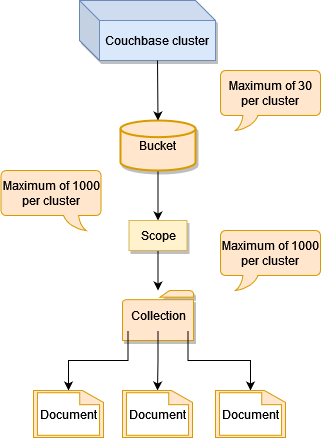
\includegraphics[scale=0.8]{images/CouchbaseArchitecture.drawio.png}
    \caption{Couchbase Architecture \parencite{CouchbaseArchitecture}}
    \label{fig:CouchbaseArchitecture}
\end{figure}
This overview of a Couchbase cluster is everything one needs to get started. The \ac{JSON} documents are stored in collections, which are put into scopes. These scopes are further put into buckets, that are the top layer of storage. \parencite{CouchbaseIntroduction}\newline
With this, one can get a personal database running, but how is it possible to scale a database to enterprise levels? A cluster consists of one or multiple interchangeable nodes, that communicate peer-to-peer and can stand alone. One node can be any computer system running the Couchbase Server system. \parencite{CouchbasePaper}\newline Each node has a Cluster Manager, which is responsible for node coordination and also acts as an interface for users to administrate the cluster. Starting out with the first node, there will be four services running:
\begin{itemize}
    \item Data Service
    \item Index Service
    \item Query Service
    \item Search Service
\end{itemize}
These services can be configured across nodes, so that a cluster can consist of four nodes with each running one of the services. Running the same service on multiple nodes is also possible. \parencite{CouchbaseIntroduction} \newline
To sum up, every node in a cluster has a cluster manager and storage as seen in (fig \ref{fig:CouchbaseArchitecture}) as well as services, that can be spread across nodes. This allows Couchbase to implement \ac{MDS} to their database, that offers the opportunity for users not only to scale-up, but also scale-out their database. \parencite{CouchbasePaper}


\section{API}
The industry evolved to support more work from home or out of office, but users still want to administrate and work on their database. This is the reason why most \ac{NoSQL} databases support an \ac{API}, which makes administrating over \ac{HTTP} possible and easy to use.\newline
Couchbase DB provides an \ac{REST} \ac{API}, that supports various functions from cluster creation to managing nodes and retrieving statistics of a database. Currently, there are thirteen different \ac{REST} \acp{API} to use. The most important ones being Nodes and Clusters \ac{API}, Buckets \ac{API}, Scopes and Collections \ac{API} and Memory and Storage \ac{API}. With these users can create and manage their clusters and set up an entire database configuring different buckets, collections and storage allocation. If the database is set up and users want to start using it, the Query Service \ac{API}, which supports \ac{N1QL} queries, or the Search Service, which provides full text searches in the database, is what they need. \parencite{CouchbaseAPI}\newline
There is much more functionality to explore with the rest of the different \acp{API}. Definitely check them out before starting with the Couchbase DB cluster.


\section{Advantages \& Disadvantages}

\section{Improvement compared to relational database design}

\section{\ac{CAP} Theorem}

Since the \ac{CAP} Theorem only takes a very superficial view of a system and cannot address specific aspects and features, it is difficult to place Couchbase in one of its three dimensions.

In a default single-cluster deployment, Couchbase can be classified as a CP system, right alongside its NoSQL-competitors MongoDB and Redis. In a single-cluster Couchbase database, consistency and partition tolerance are its most important characteristics \parencite{Ostrovsky.2015}. In case of a node failure, the Couchbase cluster will not accept writes for documents if the consistency of these documents cannot be guaranteed. This is especially useful for read and write operations on single documents.

However, in a multi-cluster deployment, Couchbase uses \ac{XDCR} to achieve availability in favor of consistency \parencite{CAPXDCR.2014}.

\ac{XDCR} allows data to be replicated across clusters. The data contained inside a source bucket is replicated to a target bucket, which primarily serves as a backup. This can be done either uni- or bidirectionally, with the latter replicating data inside the target bucket to the source bucket, thus allowing both buckets to be used to serve data. These clusters can be located in totally different data centers, which enables faster access for users and applications that are in remote locations \parencite{XDCR.20230402}.

In case of a node failure, the data located in the replicated target bucket can be used to read/write, guaranteeing high availability even though the data might not be consistent. This is called \textit{eventual consistency} \parencite{DonPintoPrincipalProductManager.2014}. All writes to the database are done asynchronously across the nodes inside the cluster, which means that different nodes might have different versions of the same data at any given time. Eventually, all nodes will converge into the same state, however the time it takes to achieve convergence can depend on many factors such as network latency, load and frequency of updates. \ac{XDCR} provides several conflict resolution mechanisms to solve problems that can arise when changes are made to the same document on multiple clusters.

\begin{figure}[H]
    \centering
        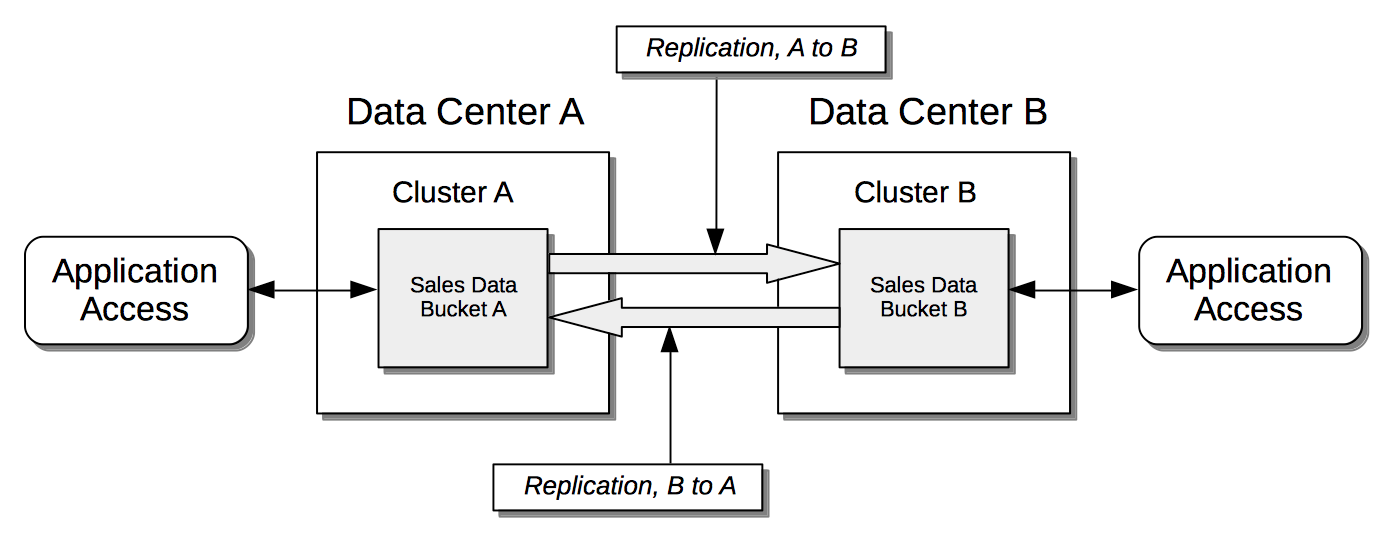
\includegraphics[scale=0.7]{images/bidirectional-xdcr.png}
    \caption{Bidirectional XDCR \parencite{XDCR.20230402}}
    \label{fig:BidiXDCR}
\end{figure}

To achieve partition tolerance, Couchbase uses its \textit{Auto Failover} feature, where nodes can be failed over automatically if they become unresponsive, so the service remains available and responsive for clients even in times of network failures\parencite{Autofailover.20230402}.

As one can see, applying the \ac{CAP} theorem to Couchbase is rather difficult since it heavily depends on its deployment method. In summary, Couchbase can be used as both a CP and AP system, with single cluster systems being configured as CP and multi cluster systems configured as an AP system. Couchbase provides mechanisms for enforcing both consistency and availability while handling network partitions and failures, so users can have a seamless experience using it.

\section{Fields of Application}

With its highly scalable and flexible nature, Couchbase has a wide range of applications in various industries. Its high-performance and features make Couchbase a good choice for web and mobile applications as well as e-commerce, finance, healthcare and gaming \parencite{CouchbaseWebsite.20230329}.

In e-commerce applications, which is the most common use case for Couchbase, it is used to store and manage user profiles, product catalogs and transactional data. It allows companies to deliver personalized shopping experiences with real-time inventory updates to their customers.

Ad tech companies use Couchbase to store and manage large amounts of data such as user profiles, ad impressions and clickstream data. It can handle high volumes of data and provides real time analytics, thus enabling ad tech companies to deliver personalized ads to their customers.

In healthcare, Couchbase is used to store and manage patient data. With its robust security and compliance features, it allows healthcare organizations to protect sensitive patient information.
 
Couchbase can work with large amounts of unstructured data and, since its schema is not fixed, can easily adapt to changing requirements. Its distributed architecture also makes it efficient in use cases regarding Internet of Things or real time Big Data \parencite{StudentCouchbase.}.

Especially companies, that want to have the benefits of NoSQL databases, but have difficulties migrating their relational database management system, use Couchbase since its \ac{N1QL} query language is very similar to the well-known \ac{SQL} language.

Overall, Couchbase is a highly versatile and scalable database that can be used in many different industries. Its fast data access, scalability and features make it a valuable tool for modern applications. Couchbase is used in many different industries by various companies such as PayPal, LinkedIn, Emirates and many more.

\section{Installation and setup of database}

\subsection{Windows}


\subsection{Docker}
If the user wants to have multiple nodes, or does not have a clean system, we recommend installing Couchbase in a Docker Container. Couchbase has an official Docker image, which can be found in the Docker Hub.

\begin{lstlisting}
docker run -d --name db -p 8091-8096:8091-8096 -p 11210-11211:11210-11211 couchbase
\end{lstlisting}


\section{Example}

\begin{figure}[H]
    \centering
        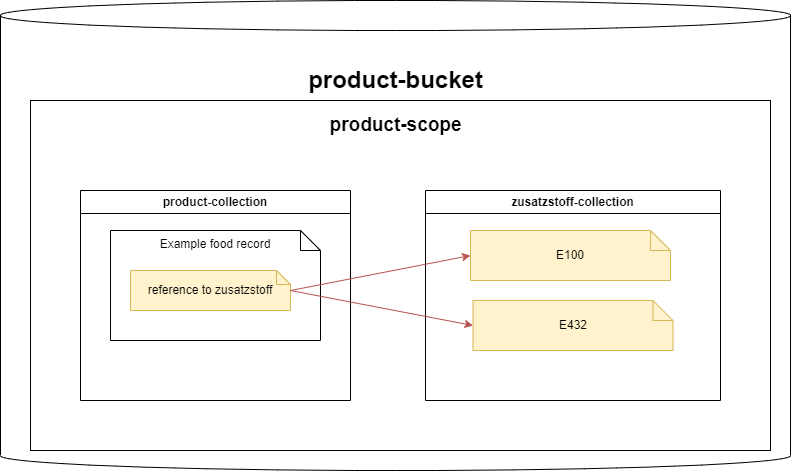
\includegraphics[height=9cm]{images/Architecture_Example_Couchbase.png}
    \caption{Couchbase Example Architecture}
    \label{fig:CouchbaseExampleArchitecture}
\end{figure}

\subsection{Query Tool}

\begin{figure}[H]
    \centering
        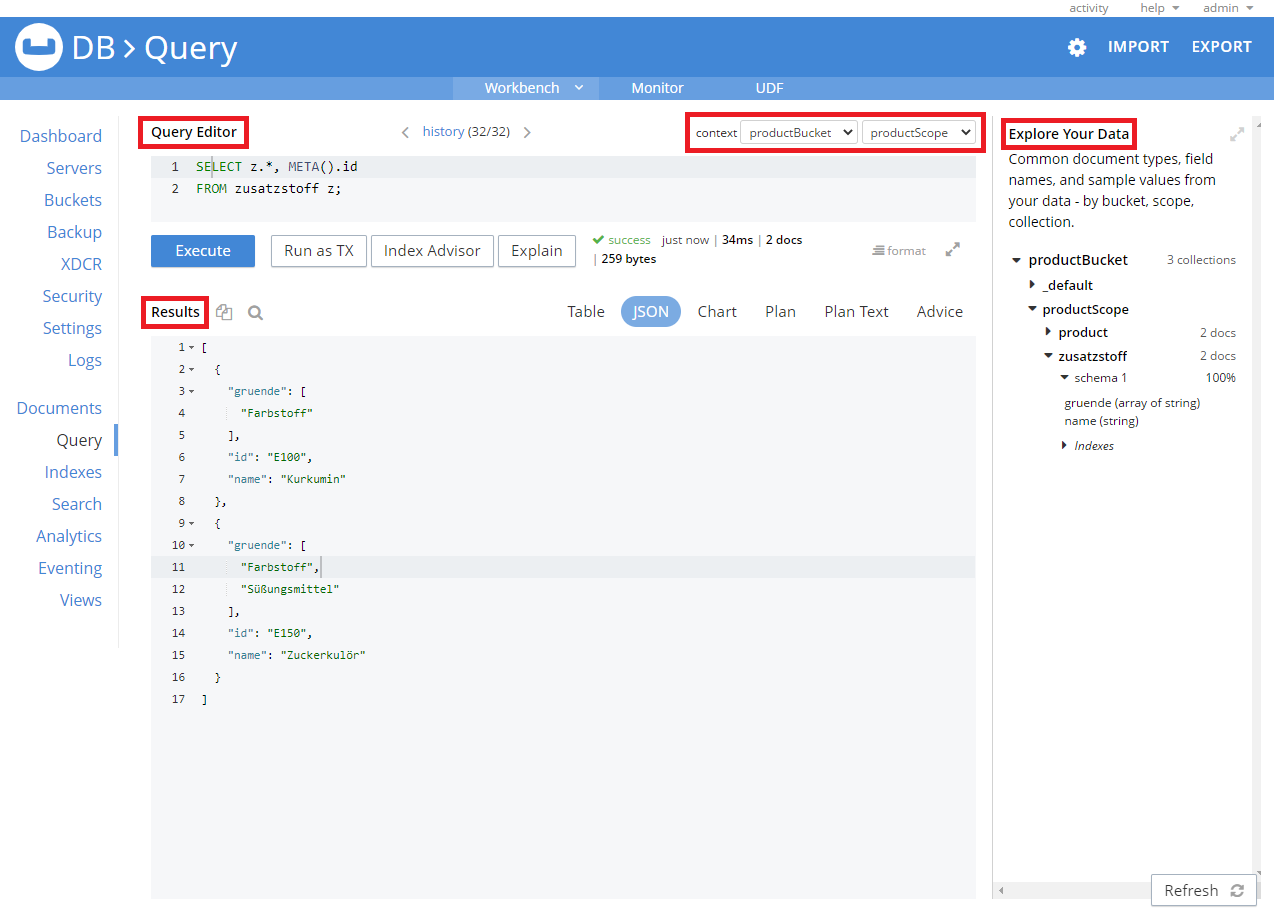
\includegraphics[height=10cm]{images/Query_Tool_Couchbase_marked.png}
    \caption{Couchbase Query Tool}
    \label{fig:CouchbaseQueryTool}
\end{figure}

Couchbase offers a Query Editor in its \ac{UI}. This tool can be used to execute queries on the database. The query has to be written in \ac{N1QL} in the editor text field. The "Execute"-button can then be used to carry out the query.

In the "Results" part, the result to the query is shown. By default, a JSON is returned, but other formats can also be chosen. 

The context drop-down menu can be used by the user to set the context where a query should be executed. The user can select the bucket and after selecting the bucket they can choose the scope. By doing this, the user eliminates the necessity to specify the path for the collections.

The "Explore Your Data" 

The Query Editor saves all the executed queries in (\cite{Couchbase.20230325})


\section{Recommendation \& Conclusion}